\newpage
{\color{gray}\hrule}
\begin{center}
\section{The Analytical Solution}
\bigskip
\end{center}
{\color{gray}\hrule}
\begin{multicols}{2}

As discussed in the previous section, the given voltage input can also be expressed as a linear combination of DC and AC voltage sources, with the help of Fourier Series.
Thus we can interpret the differential equations of the system as
%\begin{align*}
    $L\frac{di}{dt}+Ri=f(x)$
%\end{align*}
where
\begin{equation}
\begin{split}
f(x) &= 10\alpha + \sum_{n=1}^{\infty} \Bigg[ \frac{10 \sin (2 \pi n \alpha)}{\pi n} \cos\left(\frac{2\pi n}{T} x \right) \\
&+ \frac{10}{\pi n} (1 - \cos (2 \pi n \alpha)) \sin\left(\frac{2\pi n}{T} x \right) \Bigg]
\end{split}
\end{equation}

\subsection{Current Response of the Circuit for Individual Inputs}

\subsubsection{For DC Voltage Input}
Assume the current produced in the circuit by the DC source to be $i_0$
The differential equation for this system is:

\begin{align}
    \frac{di_0}{dt}+\frac{R}{L}i_0=\frac{a_0}{L}
\end{align}
Multiplying with Integrating Factor $e^{\int \frac{R}{L}dt}=e^{\frac{R}{L}t}$ and integrating on both sides with limits $t=0$ to $t=t$, and considering $i_0(0)=0$,

\begin{align}
    i_0(t)=\frac{a_0}{R} \left(1-e^{\frac{-R}{L}t} \right)
\end{align}
where $a_0=10\alpha$.

\subsubsection{For AC Voltage Input}
Assume the current produced in the circuit by the AC source  $a_ncos(n\omega_0t)+b_nsin(n\omega_0t)$ to be $i_n$.\\
The differential equation for this system is:
\begin{align}
    \frac{di_n}{dt}+\frac{R}{L}i_n=\frac{a_n}{L}cos(n\omega_0t)+\frac{b_n}{L}sin(n\omega_0t)
\end{align}
Multiplying with Integrating Factor $e^{\int \frac{R}{L}dt=e^\frac{R}{L}t}$ and integrating on both sides with limits $t=0$ to $t=t$, and considering $i_n(0)=0$,
\begin{align}
e^{\frac{R}{L}t}i_n(t) &= \int_{0}^{t} e^{\frac{R}{L}t} \left( \frac{a_n}{L}\cos(n\omega_0t) \right) dt \nonumber \\
&+ \int_{0}^{t} e^{\frac{R}{L}t} \left( \frac{b_n}{L}\sin(n\omega_0t) \right) dt \label{eq}
\end{align}
Rewriting $a_ncos(n\omega_0t)+b_nsin(n\omega_0t)$ on RHS as 
\begin{align*}
    &=a_ncos(n\omega_0t)+b_nsin(n\omega_0t)\\
    &= \sqrt{a_n^2+b_n^2} \Bigg( \frac{a_n}{\sqrt{a_n^2+b_n^2}} \cos(n\omega_0t) \\
    &+ \frac{b_n}{\sqrt{a_n^2+b_n^2}} \sin(n\omega_0t) \Bigg)\\
    &=\sqrt{a_n^2+b_n^2}\left(cos(n\omega_0t-\phi) \right)\\
    &=\sqrt{a_n^2+b_n^2}\left( \frac{e^{j(n\omega_0t-\phi)}+e^{j(\phi-n\omega_0t)}}{2}\right)
\end{align*}
where $\phi=tan^{-1}\left(\frac{b_n}{a_n} \right)$ and substituting it back in (\ref{eq}), on RHS side we get
\begin{align}
    &=\frac{\sqrt{a_n^2+b_n^2}}{2L}\int_{0}^{t}\left( e^{\frac{R}{L}t+j(n\omega_0t-\phi)} + e^{\frac{R}{L}t+j(\phi-n\omega_0t)} \right)
\end{align}
After integrating, we get
\begin{align}
e^{\frac{R}{L}t}i_n(t) &= \frac{\sqrt{a_n^2+b_n^2}}{2L} \Bigg( \frac{e^{-j\phi}\left(e^{(\frac{R}{L}+jn\omega_0)t}-1 \right)}{\frac{R}{L}+jn\omega_0} \\
&+ \frac{e^{j\phi}\left(e^{(\frac{R}{L}-jn\omega_0)t}-1\right)}{\frac{R}{L}-jn\omega_0} \Bigg)
\end{align}
By rearranging the terms and simplifying, we get
\begin{align}
i_n(t) &= \frac{\sqrt{a_n^2+b_n^2}}{\sqrt{R^2+(n\omega_0L)^2}} \cos(n\omega_0t-\phi-\theta) \\
&- e^{\frac{-R}{L}t} \frac{\cos(\phi+\theta)}{\sqrt{R^2+(n\omega_0L)^2}}
\end{align}
where 
\begin{align*}
    \theta&=tan^{-1}\left(\frac{n\omega_0L}{R}\right)\\
    a_n&=\frac{10 \sin 2 \pi n \alpha}{\pi n} \\
    b_n&=\left( \frac{10}{ \pi n} \right) (1 - \cos 2 \pi n \alpha)
\end{align*}


\subsection{Combined Current Response (Exploiting Linearity Property)}
Since the first-order circuit is linear, we have by the principle of superposition:
 \begin{align}
        i(t) = i_0(t)+ \sum_{n=1}^{\infty}i_n(t)
\end{align}
\begin{align}
i(t) &= \frac{a_0}{R} \left(1-e^{\frac{-R}{L}t} \right) \\
&+ \sum_{n=1}^{\infty} \Bigg( \frac{\sqrt{a_n^2+b_n^2}}{\sqrt{R^2+(n\omega_0L)^2}} \cos(n\omega_0t-\phi-\theta) \\
&- e^{\frac{-R}{L}t} \frac{\cos(\phi+\theta)}{\sqrt{R^2+(n\omega_0L)^2}} \Bigg)
\end{align}
where
\begin{align*}
    a_0&=10\alpha\\
    \theta&=tan^{-1}\left(\frac{n\omega_0L}{R}\right)\\
    a_n&=\frac{10 \sin 2 \pi n \alpha}{\pi n} \\
    b_n&=\left( \frac{10}{ \pi n} \right) (1 - \cos 2 \pi n \alpha)
\end{align*}


\subsection{Visual Representation of the Response}
\begin{figure}[H]
  \centering
  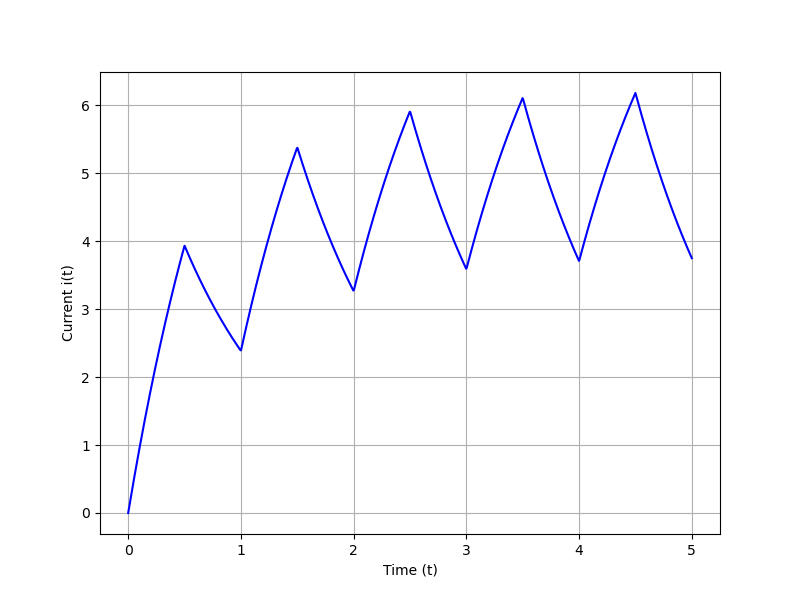
\includegraphics[width=\columnwidth]{sections/3_plot.png}
  \caption{Current Response for $R=1\Omega$, $L=1H$, and $\alpha=0.5$}
  \end{figure}
\end{multicols}
